% -*- TeX:UK -*-
\documentclass[10pt]{beamer}
\usetheme{metropolis}
%\useinnertheme{rectangles}
\setbeamercovered{%
still covered={\opaqueness<1->{15}},
again covered={\opaqueness<1->{40}}}

\hypersetup{colorlinks,linkcolor=black,urlcolor=brown,citecolor=brown}

\usepackage{amsmath,amssymb,amsthm}
\usepackage{unicode-math}

% We set the Lucida OTF fonts as default
\usepackage{fontspec}
\setmainfont{Lucida Bright OT}
\setsansfont{Lucida Sans OT}
\setmonofont{Lucida Console DK}[Scale=MatchLowercase]

\newfontfamily\webglyphsfont{WebHostingHub-Glyphs}[Scale=0.7]
\newcommand\webglyphs[1]{{\webglyphsfont\symbol{#1}}}
\newcommand\Discussion{\colorbox{white}{\textcolor{black}{\webglyphs{"F134}}}\xspace}
\newcommand\DiscussionI{\colorbox{black}{\textcolor{white}{\webglyphs{"F134}}}\xspace}
\newcommand\DExamples{\colorbox{black}{\textcolor{white}{\webglyphs{"F134} examples?}}}
\newcommand\Reading{\colorbox{black}{\textcolor{white}{\webglyphs{"F0C1}}}\xspace}
\newcommand\ReadingI{\colorbox{white}{\textcolor{black}{\webglyphs{"F0C1}}}\xspace}
\newcommand\Video{\colorbox{white}{\textcolor{black}{\webglyphs{"F03D}}}\xspace}
\newcommand\Attention{\colorbox{black}{\textcolor{orange}{\webglyphs{"F05A}}}\xspace}
\newcommand\HomeWork{\colorbox{white}{\textcolor{black}{\webglyphs{"F5ED}}}\xspace}
\newcommand\HomeWorkI{\colorbox{black}{\textcolor{white}{\webglyphs{"F5ED}}}\xspace}
\newcommand\Advanced{\colorbox{black}{\textcolor{white}{\webglyphs{"F235}}}\xspace}

\newfontfamily\lineabasicfont{linea-basic-10}
\newcommand\basicicons[1]{{\lineabasicfont\symbol{#1}}}
\newcommand\timeforwards{\basicicons{"0079}}
\newcommand\timebackwards{\basicicons{"0064}}

\newfontfamily\lineaweatherfont{linea-weather-10}
\newcommand\weathericons[1]{{\lineaweatherfont\symbol{#1}}}
\newcommand\meteosun{\weathericons{"E038}}
\newcommand\meteosuncloud{\weathericons{"E042}}
\newcommand\meteorain{\weathericons{"E033}}
\newcommand\meteowind{\weathericons{"E054}}

\newfontfamily\uleaffont{Mini Pics Uprooted Leaf}
\newcommand\uleafmpics[1]{{\uleaffont\symbol{#1}}}
\newcommand\lowplants{\uleafmpics{"00CE}}
\newcommand\mediumplant{\uleafmpics{"006A}}
\newcommand\bush{\uleafmpics{"0039}}
\newcommand\smallplant{\uleafmpics{"0030}}
\newcommand\seedling{\uleafmpics{"002F}}
\newcommand\floweringplant{\uleafmpics{"00CA}}

\newfontfamily\utwigfont{Mini Pics Uprooted Twig}
\newcommand\utwigmpics[1]{{\utwigfont\symbol{#1}}}
\newcommand\grassplant{\utwigmpics{"0033}}

\newfontfamily\uinsectfont{Insect Icons}
\newcommand\uinsect[1]{{\uinsectfont\symbol{#1}}}
\newcommand\bug{\uinsect{"006F}}

\usepackage{polyglossia}
\setdefaultlanguage[variant = british, ordinalmonthday = false]{english}

\usepackage[style=authoryear-comp,firstinits,sortcites,maxcitenames=2,%
    mincitenames=1,maxbibnames=10,minbibnames=10,uniquename=mininit,%
    uniquelist=minyear,sortfirstinits=true]{biblatex}
\addbibresource{../references/ecophys.bib}
\renewcommand{\bibfont}{\small}

\usepackage{abbrev}



\usepackage{tikz}
\usetikzlibrary{positioning,fit,arrows}

\tikzset{
 big dot/.style
  = {circle, draw, inner sep=0pt, minimum size=3mm, fill=teal!50},
 a/.style
  = {node distance=4em, text width=0.1em, minimum height=4em},
 b/.style
  = {rectangle, draw, fill=gray!10, node distance=4em, text width=6em,
     text centered, rounded corners, minimum height=4em, thick},
 c/.style
  = {circle, draw, dashed, fill=orange!10, inner sep = 0pt, node distance=5em, text width=6em,
     text centered, thick},
 d/.style
  = {rectangle, draw, dashed, fill=red!10, node distance=4em, text width=6em,
     text centered, rounded corners, minimum height=4em, thick},
 l/.style
  = {draw, -latex, ultra thick},
 lr/.style
  = {draw, latex-latex, ultra thick, red},
 lb/.style
  = {draw, -latex, ultra thick, blue},
  lo/.style
  = {draw, -latex, ultra thick, orange},
  lg/.style
  = {draw, -latex, ultra thick, teal},
  mylabel/.style
  ={text width=6.5em, text centered},
 aa/.style
  = {node distance=4em, text width=0em, minimum height=0.5ex},
 ll/.style
  = {draw, {open triangle 45} -, thick},
 llb/.style
  = {draw, - triangle 45, thick, blue},
 llg/.style
  = {draw, - open triangle 45, thick, green},
  llt/.style
  = {draw, - open triangle 45, thick, teal},
 llr/.style
  = {draw, - triangle 45, thick, purple},
 llo/.style
  = {draw, - triangle 45, thick, orange}
}

\begin{document}

\title{IPS-141\\Sensory and Physiological\\Ecology of  Plants}
\subtitle{1: Introduction}
\author{Pedro J. Aphalo}
\date{January--February 2022}
\institute[Univ.\ of Helsinki]{M.Sc.\ in Integrative Plant Science, University of Helsinki\\[2ex] \url{http://blogs.helsinki.fi/aphalo/}\\[2ex] \url{mailto:pedro.aphalo@helsinki.fi}}


  \begin{frame}
    \maketitle
  \end{frame}

  \begin{frame}[c]
    \begin{center}
      \begin{small}
        \copyright 2006--2022 by Pedro J. Aphalo\\
        University of Helsinki, Finland.\\
        \textcolor{blue}{\url{http://blogs.helsinki.fi/senpep-blog/}}\\[2ex]
      \end{small}

      \begin{footnotesize}
        Sensory and Physiological Ecology of Plants slides by Pedro J. Aphalo are licensed under a Creative Commons Attribution-ShareAlike 4.0 International License.

      
\includegraphics[width=6em]{../figures/copyright/by-sa}\\[2ex]
      \end{footnotesize}
        
        \begin{scriptsize}
        Typeset in Lucida Sans, \textrm{Luicda Bright}, \texttt{Lucida Console} and Lucida Math. Icons from fonts ``WebHostingHub Glyphs'' (under SIL-Open Font License) from \url{https://www.webhostinghub.com/}; ``insect icons'' (free from \url{http://www.woodcutter.es/}); ``linea-basic-10'' and ``linea-weather-10'' (free from \url{https://github.com/linea-io}), ``Mini Pics Uprooted Twig'' and ``Mini Pics Uprooted Twig'' (commercial, from Image Club Graphics, Inc.). Plant icon as .svg by Abdul Wahhab (free from \url{NounProject.com}).

        Illustrations and text quoted from copyrighted sources is excluded from this license and their use should respect the original licenses.
        \end{scriptsize}
    \end{center}
  \end{frame}


  \begin{frame}
    \frametitle{Outline}
    \tableofcontents
  \end{frame}

\section{Introductions}

\begin{frame}{Let's introduce ourselves \Discussion}
  \begin{itemize}
    \item Name
    \item Subject of study and background
    \item Are you interested in the subject of the course?
    \item What do you expect to learn?
    \item Anything else relevant
  \end{itemize}
\end{frame}

\section{Course organization}

\begin{frame}{Zoom and Moodle}
\begin{itemize}
  \item Due to COVID our learning space is virtual.
  \item Let's all together keep interaction active.
  \item Short lectures interspersed with discussion in groups.
  \item Feel free to ask any questions or challenge what I present.
  \item Photo in profile/video and Zoom recordings.
  \item Moodle: \url{https://moodle.helsinki.fi/index.php?id=48992}
\end{itemize}
\end{frame}

\section{Motivation: scaling up or down}

\begin{frame}{\emph{Vicia faba} and ``drought'' $\times$ genotype}
  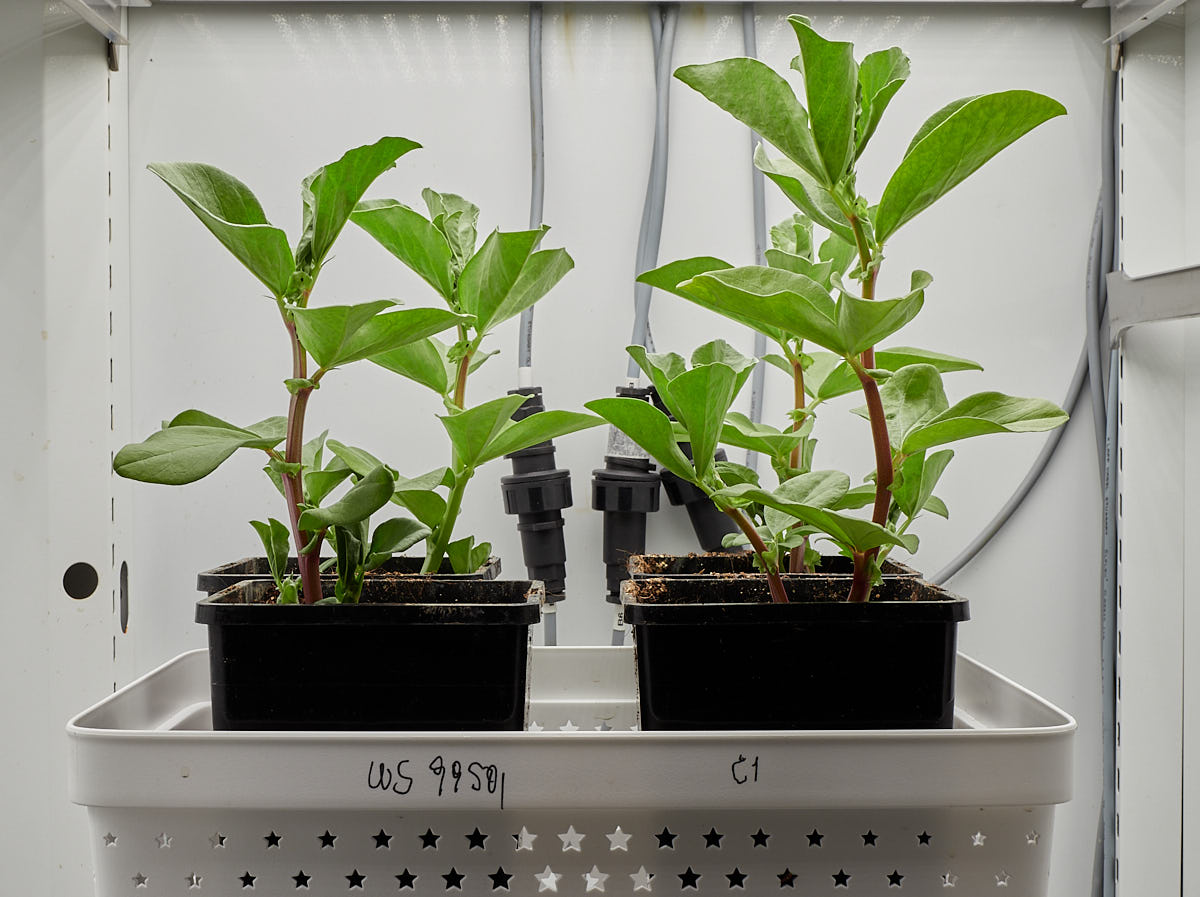
\includegraphics[width=0.40\linewidth]{photos/v-faba-WS-before}\hfil
  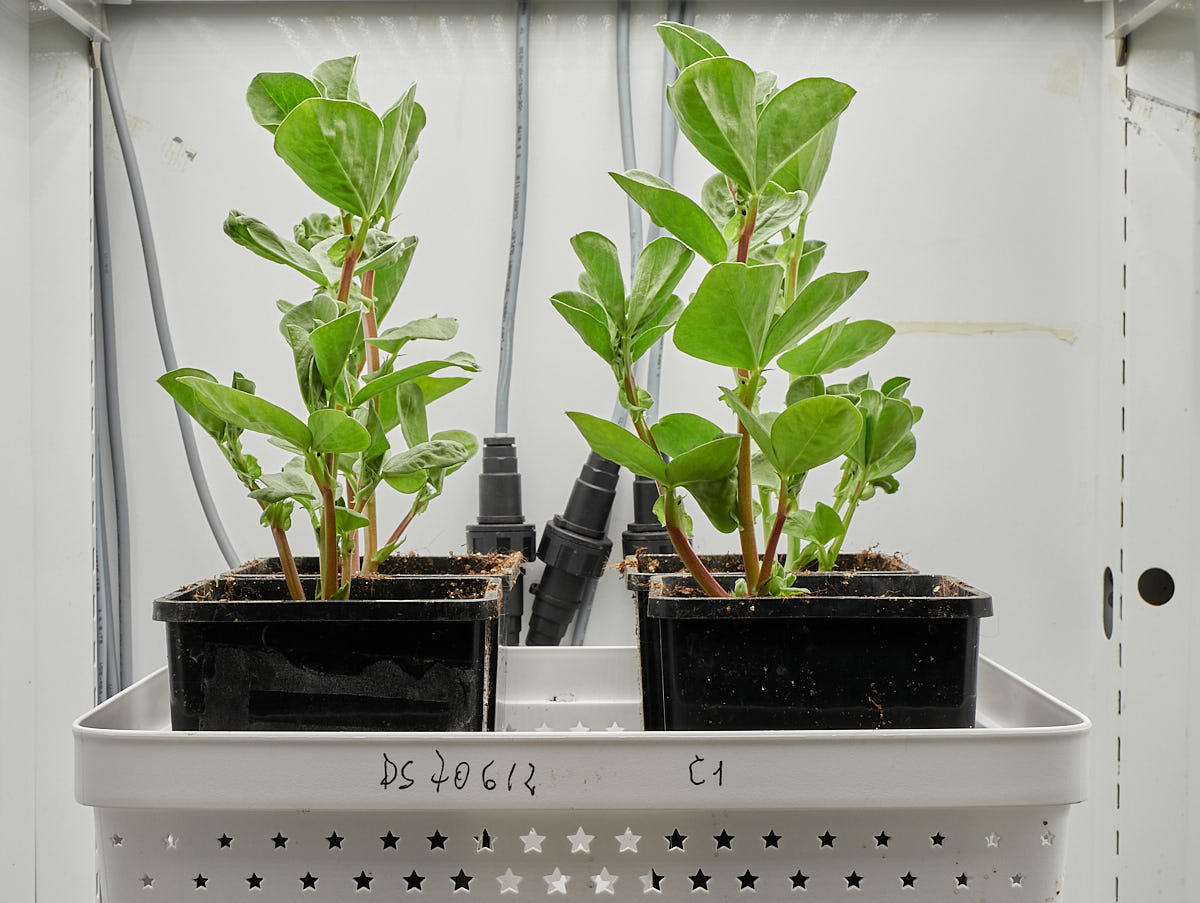
\includegraphics[width=0.40\linewidth]{photos/v-faba-DS-before}\\
  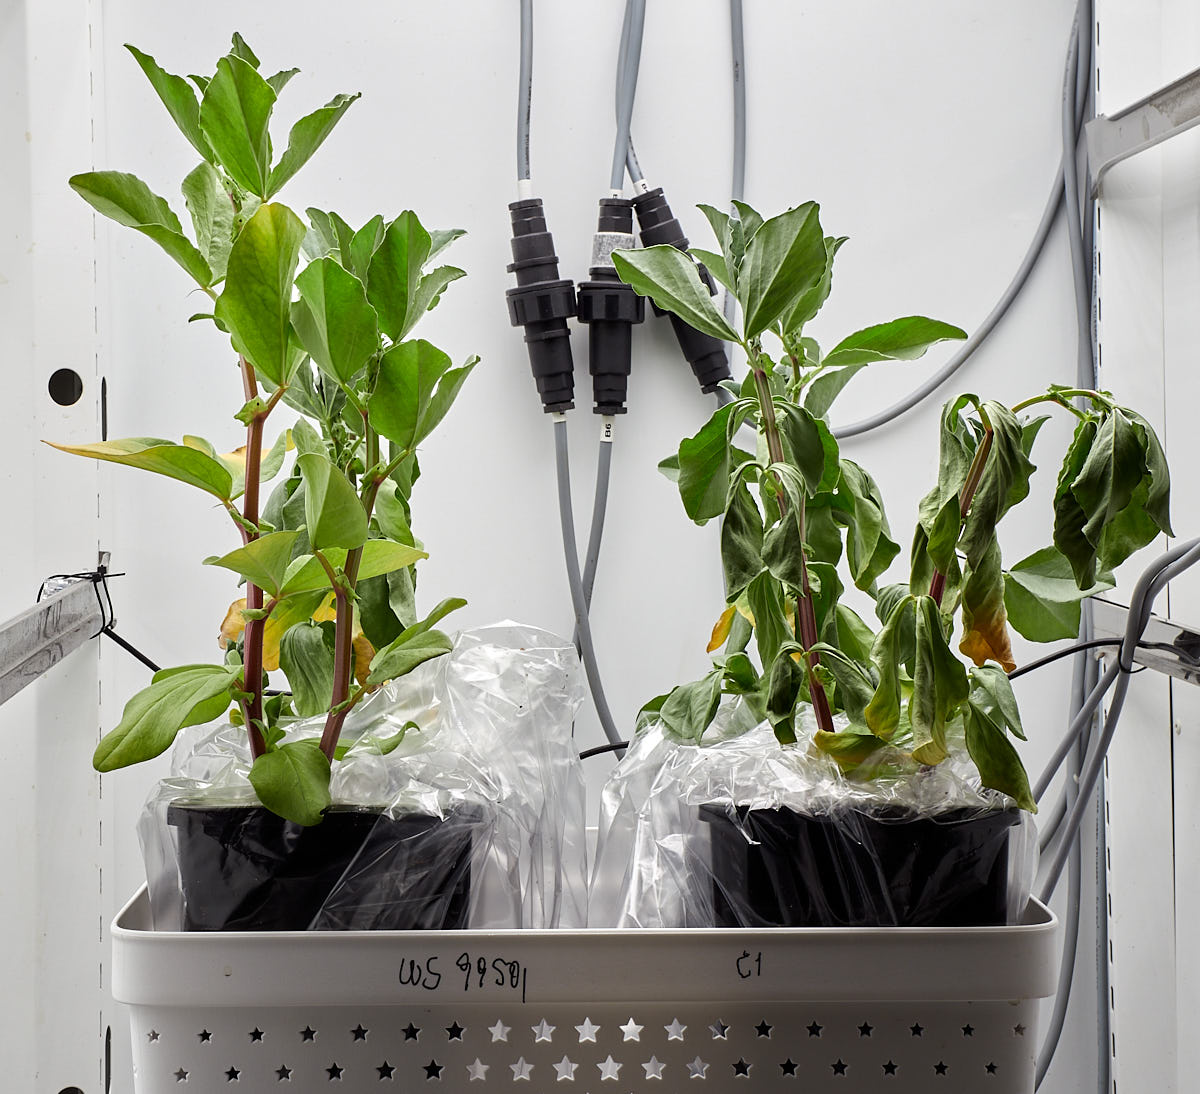
\includegraphics[width=0.40\linewidth]{photos/v-faba-WS-after}\hfil
  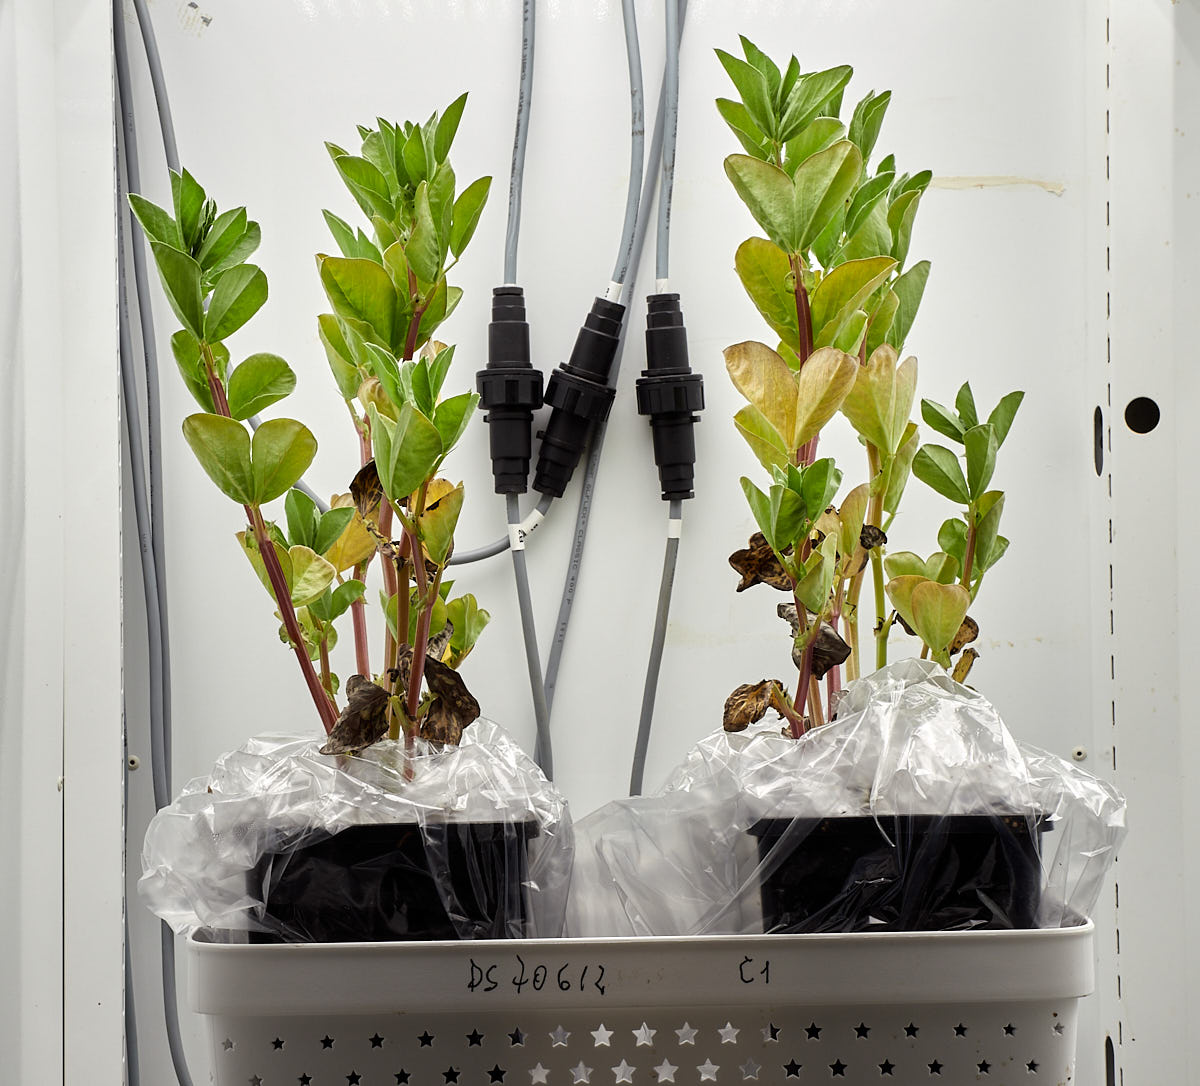
\includegraphics[width=0.40\linewidth]{photos/v-faba-DS-after}
\end{frame}

\begin{frame}{Vegetation}
  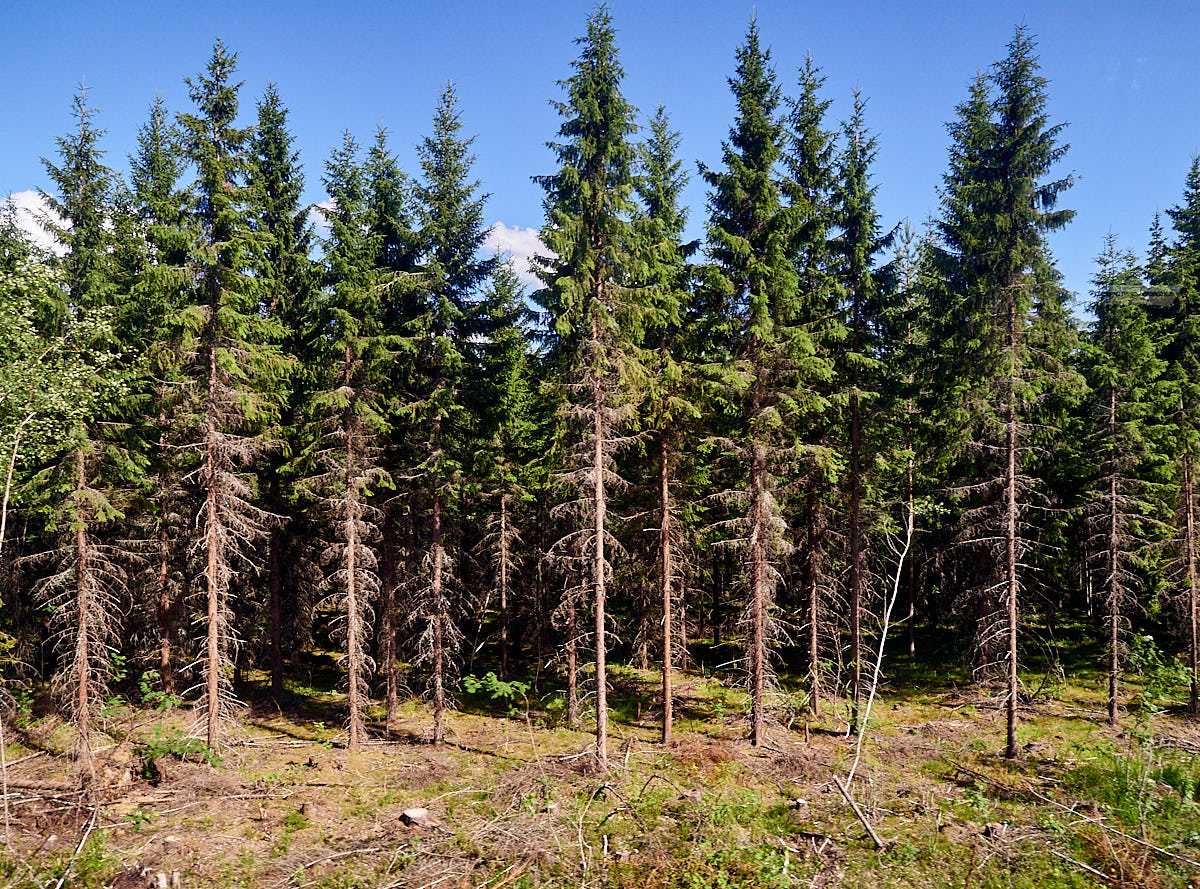
\includegraphics[width=0.47\linewidth]{photos/spruce-forest}\hfil
  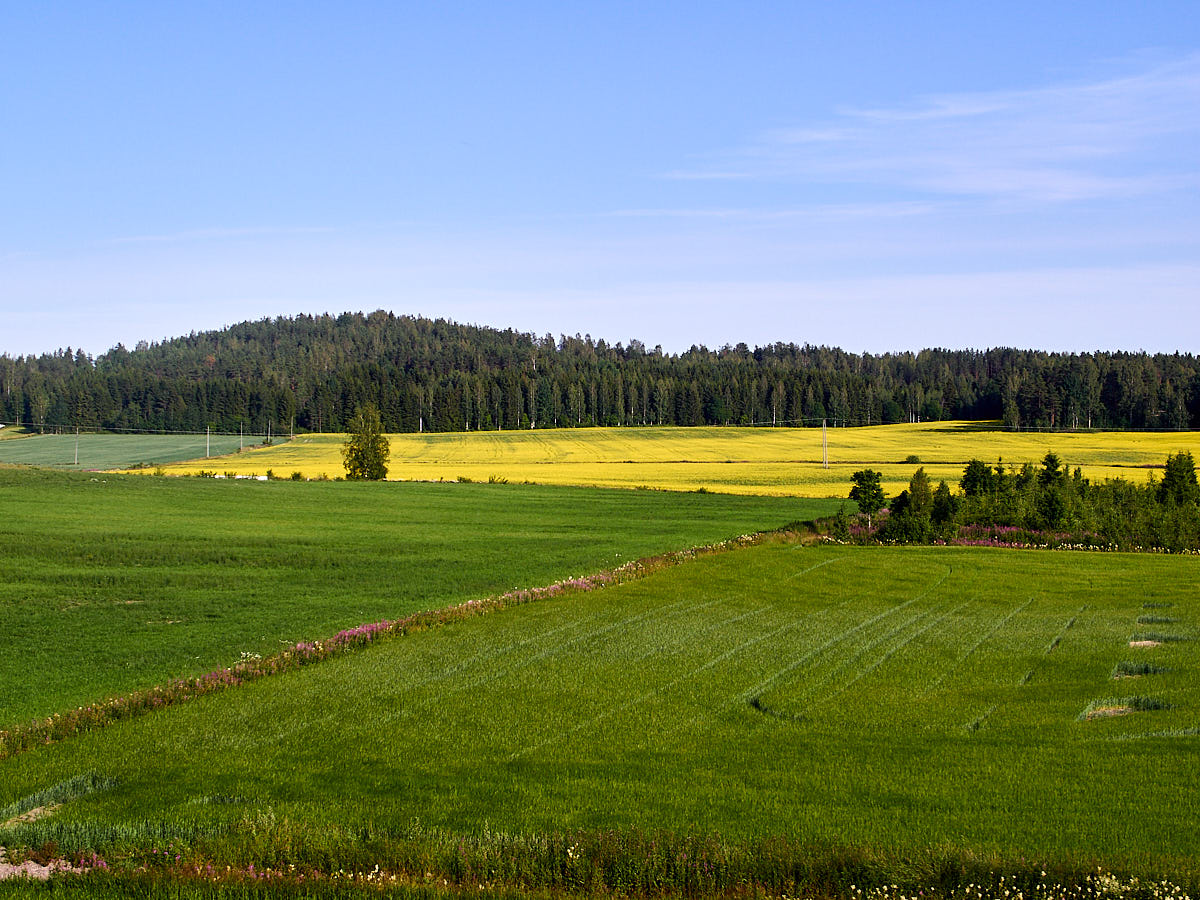
\includegraphics[width=0.47\linewidth]{photos/fields}\\
  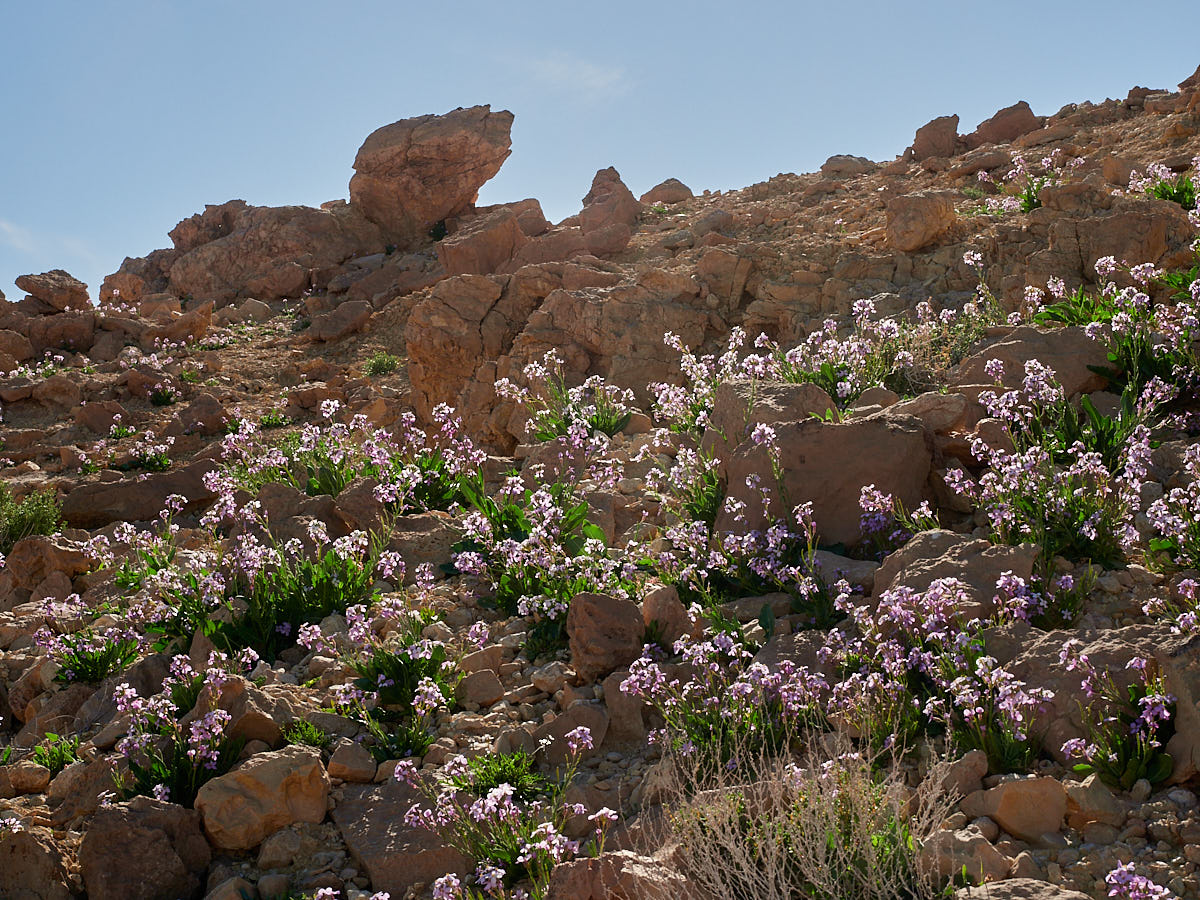
\includegraphics[width=0.47\linewidth]{photos/negev-1}\hfil
  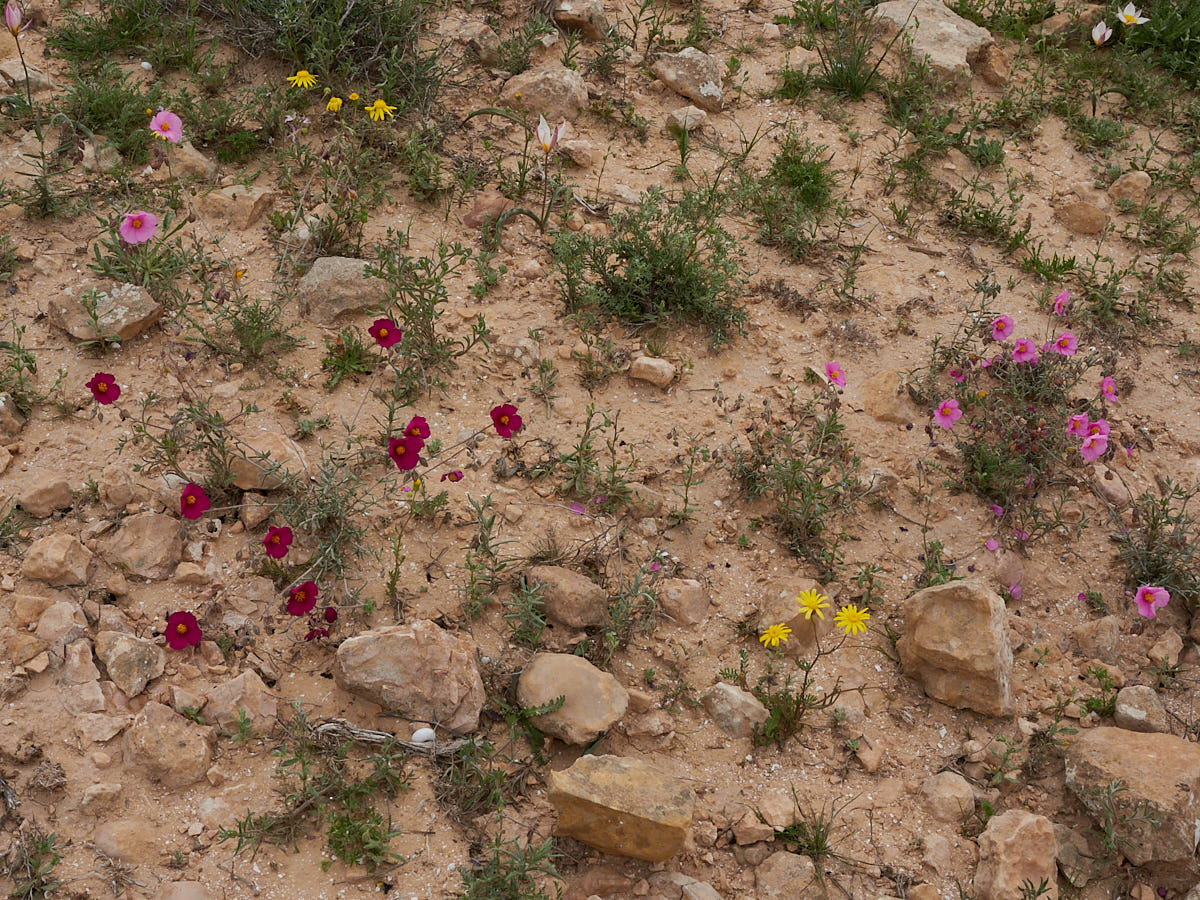
\includegraphics[width=0.47\linewidth]{photos/negev-2}
\end{frame}

\begin{frame}{A systems view of the living world}
  \begin{itemize}
    \item Many interactions $\Rightarrow$ structural complexity
    \item Many feedback loops $\Rightarrow$ complex dynamics
    \item Complexity $\Rightarrow$ emergent properties
    \item \ldots emergent properties cannot be predicted directly
    \item \Attention cellular processes are not enough predict plant responses
    \item \Attention individual plant responses are not enough to predict community behaviour/crop performance
    \item \DiscussionI Can you think of specific examples?
    \item \emph{We will focus on the role interactions and how plants
    exploit them and the connection between interactions and evolution}
  \end{itemize}
\end{frame}

\begin{frame}{Some of the recent advances in plant researcch}
   \begin{itemize}
     \item Synchronization of behaviour among individual plants
     \item Anticipatory responses to future conditions
     \item Strategies such as risk avoidance and bet-hedging vs.\ tolerance
     \item Role of correlations in the environment in plant responses
     \item ``Darwinian agriculture''
     \item Implications of complexity of regulation for genetic manipulation
     \item Big data, machine learning\ldots
   \end{itemize}
\end{frame}

\section{Why \emph{sensory and physiological ecology}?}

\begin{frame}{Changing perspective in Biology + \Discussion}
  \begin{description}
    \item[Era: Industrial revolution] Organisms studied as mechanical machines. Chemistry and Physics provide mechanisms.
    \item[Era: Information revolution] Organisms viewed as processors of information. We add a new layer of explanation on top of earlier ones.
    \item[Animals vs.\ plants] The role of information in animals was recognized earlier than in plants.
    \item[\DiscussionI] Examples?
  \end{description}
\end{frame}

\begin{frame}{Physiology vs.\ ecology (typical definitions)}
    \textbf{Plant physiology} is the study of the function,
    or physiology, of plants. Fundamental processes such as
    photosynthesis, respiration, plant nutrition, water
    relations, and development are studied by plant physiologists.\\[2ex]

    \textbf{Plant ecology} is the study of the factors affecting the distribution and abundance
    of plants. It aims to show how pattern and structure at
    different levels of organization are influenced by abiotic
    factors (e.g.\ climate and soil) and biotic interactions
    (e.g.\ competition, facilitation, symbiosis and parasitism)
    \\  \vspace{\stretch{1}}
\end{frame}

\begin{frame}{Ecology's subdisciplines}
    \Attention Boundaries can be fuzzy!

    \begin{itemize}
        \item[$\blacktriangleright$] \emph{Physiological ecology} and
        Behavioural ecology examine adaptations of the individual
        to its environment.
        \item[$\blacktriangleright$] \emph{Sensory ecology} studies how individuals acquire, process, and respond to information from their environment.
        \item[$\blacktriangleright$] \emph{Evolutionary ecology} explicitly considers the evolutionary histories of species.
        \item[$\vartriangleright$] \emph{Population ecology (or autecology)} studies the dynamics of populations of a single species.
        \item[$\vartriangleright$] \emph{Community ecology (or synecology)} focuses on the interactions between species within a community.
        \item[$\vartriangleright$] \emph{Ecosystem ecology} studies the flows of energy and matter through the biotic and abiotic components of ecosystems.
        \item[$\vartriangleright$] \emph{Landscape ecology} examines processes and relationships across multiple ecosystems or very large geographic areas.
    \end{itemize}

\end{frame}

\begin{frame}{Physiological ecology/Stress physiology}
    \begin{itemize}
        \item Viewpoint: plants as ``victims'' of the environment.
        \item \emph{Physiological ecology $\approx$ ecophysiology} seeks to describe the
        \textbf{physiological mechanisms} that underlie ecological
        observations.
        \item \emph{Stress physiology} differs only by its focus on extreme environmental conditions instead of all conditions.
        \item \emph{Ecophysiologists address ecological questions about
        the controls over growth, reproduction, survival, abundance,
        and geographical distribution of plants as these processes
        are affected by the ``mass + energy'' exchange between plants and their
        physical, chemical, and biotic environment.}
    \end{itemize}
\end{frame}

\begin{frame}{Sensory ecology}
    \begin{itemize}
        \item Viewpoint: plants as ``navigators'' in the environment.
        \item Sensory ecology studies the \textbf{mechanisms of information acquisition and emission}
        that underlie ecological observations.
        \item \emph{Sensory ecologists address ecological questions about
        the controls over growth, reproduction, survival, abundance,
        and geographical distribution of plants as these processes
        are affected by the ``information'' exchange between plants and their
        physical, chemical, and biotic environment.}
    \end{itemize}
\end{frame}

\begin{frame}{Fitness and evolution}
    \Attention ``Nothing makes sense in Biology except in the light of evolution''

    \vspace{0.5ex}
       \emph{Fitness} is ``measured'' as the success in producing viable offspring (passing genes to the next generation).

       The organisms we study are the result of the \emph{evolutionary process}. To understand why organisms have the functions, morphology, life cycle and behaviour they have, we need to take into account how these features contribute to fitness.

       These functions include both sensing leading to development ``decisions'' and regulation of metabolism and growth supporting reproduction and/or multiplication, and thus fitness.
\end{frame}

\begin{frame}{Cause and effect in Biology \Discussion 10 + 5 min}

\begin{centering}
$\to$ \emph{fitness} $\to$ genome $\to$  epigenome $\to$ phenome $\to$ \emph{fitness} $\to \cdots$
\vspace{3ex}
\end{centering}

\begin{description}
%  \item[time sequence] .
  \item[\DiscussionI] Which transitions, shown as $\to$, depend directly on the environment?
  \item[\DiscussionI] ``Evolution determines physiology'' or ``Physiology determines fitness''?
  \item[\Attention] The course of evolution is not the result of natural selection alone!
\end{description}
\pause
\Attention \emph{Multiple viewpoints are possible, and not necessarily contradictory!}
\end{frame}

\begin{frame}{Natural and artificial selection \Discussion}
  \begin{alertblock}{Crop breeding \DiscussionI 10 + 5 min}
    \begin{itemize}
      \item What is the role of artificial selection in crop breeding?
      \item What is the role of natural selection in crop breeding?
      \item Chose a crop you are familiar to explain your answers.
    \end{itemize}
  \end{alertblock}
Discuss this topic in groups of 2 or 3 students (10 min). Take notes while discussing and have them ready for general discussion (5 min).
\end{frame}

\begin{frame}{Wild plants vs.\ weeds vs.\ crops \Discussion}
    \begin{itemize}

        \item<1,4> Most \textbf{crops} have been under artificial selection for a
        long time. Farmers and breeders have selected the most useful
        genotypes.

        \item[{\small +}]<1,4> In addition natural selection is also active on cultivated plants,
        although in a managed environment. \DExamples

        \item[{\small --}]<1,4> Most crops have very low fitness in the wild. \DExamples

        \item<2,4> Crop \textbf{weeds} are not subject to artificial selection,
        they are under natural selection but in a managed environment. \DExamples

        \item<3,4> Natural selection in most populations of \textbf{wild plants} is affected by human activities. \DExamples
    \end{itemize}
\end{frame}

\begin{frame}{Adaptation vs.\ acclimation}

\begin{description}
\item[Adaptation] Genetic variation + natural selection. It takes place
over more than one generation. \textit{There is change in the
genotype}.

\item[Acclimation] Regulation within the lifetime of an individual, it
involves changes in the phenotype in response to the environment.
\textit{There is no change in the genotype}.
\end{description}

\footnotesize
\resizebox{\linewidth}{!}{%
  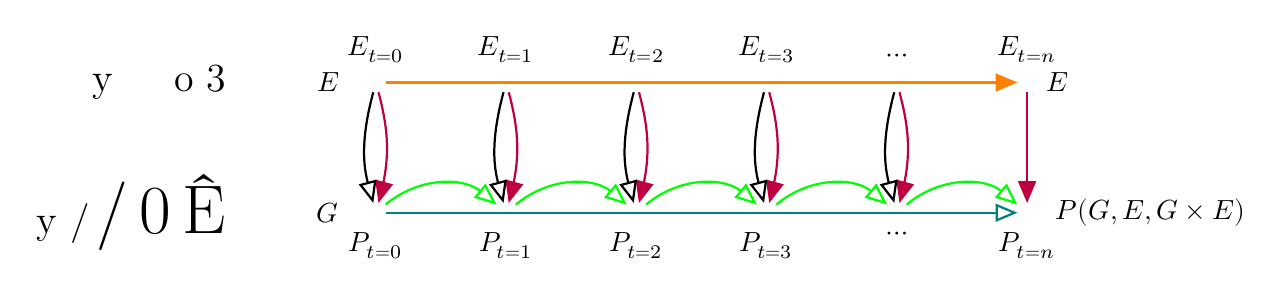
\begin{tikzpicture}[auto]
    \node [aa, label=left:{\Large\timeforwards~\meteosuncloud~\meteorain~\bug~\grassplant}] (environment) {};
    \node [aa, below = of environment, label=left:{\Large\timeforwards~\seedling\,\Huge\seedling\,\smallplant\,\floweringplant}] (plant) {};
    \node [aa, right = of environment, label=above:{$E_{t=0}$}, label=left:{$E\ \ $}] (env_zero) {};
    \node [aa, right = of env_zero, label=above:{$E_{t=1}$}] (env_one) {};
    \node [aa, right = of env_one, label=above:{$E_{t=2}$}] (env_two) {};
    \node [aa, right = of env_two, label=above:{$E_{t=3}$}] (env_three) {};
    \node [aa, right = of env_three, label=above:{$\cdots$}] (env_four) {};
    \node [aa, right = of env_four, label=above:{$E_{t=n}$}, label=right:{$E$}] (env_end) {};
    \node [aa, below = of env_zero, label=below:{$P_{t=0}$}, label=left:{$G\ \ $}] (pheno_zero) {};
    \node [aa, below = of env_one, label=below:{$P_{t=1}$}] (pheno_one) {};
    \node [aa, below = of env_two, label=below:{$P_{t=2}$}] (pheno_two) {};
    \node [aa, below = of env_three, label=below:{$P_{t=3}$}] (pheno_three) {};
    \node [aa, below = of env_four, label=below:{$\cdots$}] (pheno_four) {};
    \node [aa, below = of env_end, label=below:{$P_{t=n}$}, label=right:{\ $P(G, E, G \times E)$}] (pheno_end) {};

    \path [llo, below] (env_zero) -- (env_end);
    \path [llt, above] (pheno_zero) -- (pheno_end);

    \path [llr] (env_zero) edge [bend right=-15] (pheno_zero);
    \path [ll] (pheno_zero) edge [bend right=-15] (env_zero);
    \path [llg, above] (pheno_zero) edge [bend right=-40] (pheno_one);

    \path [llr] (env_one) edge [bend right=-15] (pheno_one);
    \path [ll] (pheno_one) edge [bend right=-15] (env_one);
    \path [llg, above] (pheno_one) edge [bend right=-40] (pheno_two);

    \path [llr] (env_two) edge [bend right=-15] (pheno_two);
    \path [ll] (pheno_two) edge [bend right=-15] (env_two);
    \path [llg, above] (pheno_two) edge [bend right=-40] (pheno_three);

    \path [llr] (env_three) edge [bend right=-15] (pheno_three);
    \path [ll] (pheno_three) edge [bend right=-15] (env_three);
    \path [llg, above] (pheno_three) edge [bend right=-40] (pheno_four);

    \path [llr] (env_four) edge [bend right=-15] (pheno_four);
    \path [ll] (pheno_four) edge [bend right=-15] (env_four);
    \path [llg, above] (pheno_four) edge [bend right=-40] (pheno_end);

    \path [llr] (env_end) -- (pheno_end);

  \end{tikzpicture}%
}%

\textrm{\textbf{Figure:} Time course of one realization of the environment ($E$) during the lifetime of an individual of a genotype ($G$) resulting in a phenotype ($P$).}
\end{frame}

\begin{frame}{Adaptation vs.\ acclimation \Discussion 5 min}

\textbf{Examples of adaptation}

Shade $\rightarrow$ larger and thinner leaves.\\
Drought $\rightarrow$ larger root:shoot weight ratio.\\
Hot + dry environment $\rightarrow$ CAM photosynthesis.\\[2ex]

\textbf{Examples of acclimation}

Shade $\rightarrow$ larger and thinner leaves.\\
Drought $\rightarrow$ larger root:shoot weight ratio.\\
Hot + dry environment $\rightarrow$ CAM photosynthesis.\\[2ex]
\pause

\DiscussionI \emph{How is it possible that the examples can be the same? Where is the difference?}

\end{frame}

\begin{frame}{You are a seed in the soil \Discussion 10 + 10 min}

Discuss this topic in groups of 2 or 3 students (10 min). Take notes while discussing and have them ready for general discussion (10 min).

\begin{alertblock}{Thought exercise: when should I germinate?}
\begin{enumerate}
  \item Write a list of dangers you are exposed to.
  \item Write a list of good opportunities you have.
  \item Write a list of conditions you can perceive around you.
  \item What information can you obtain?
  \item How would you use this information to decide to germinate of not?
\end{enumerate}
\end{alertblock}

\end{frame}

\section{Plants and animals}

\begin{frame}{Plants $\neq$ animals}

\center
\begin{tabular}{lll}
\hline
& \textbf{Plants} & \textbf{Animals}\\
\hline
Mobility & sessile & mobile\\
Structure & modular & fixed\\
Growth & indeterminate & determinate\\
Energy source & light & organic substances\\
\hline
\end{tabular}
%\vspace{5mm}
\end{frame}

\begin{frame}{Plants $\approx$ animals}

\center
\begin{tabular}{lll}
\hline
& \textbf{Plants} & \textbf{Animals}\\
\hline
Structure & complex & complex\\
Function & complex  & complex\\
Behaviour & complex & complex\\
Sensing & yes & yes\\
Communication & `yes' & yes\\
Memory & `yes' & yes\\
Problem solving & `yes' & yes\\
Learning & `yes' & yes\\
\hline
\end{tabular}
\end{frame}

\begin{frame}{Challenges for research + \Discussion}

\begin{itemize}
    \item<1-2> We need to recognize very different ways of behaving, communicating, and perceiving compared to our own.
    \item<1-2> We should avoid projecting our own human image on the behaviour we observe in plants.
    \item<1-2> We should analyse characteristics and behaviour in relation to life history and fitness.
\end{itemize}

\begin{alertblock}<2>{Plants' `senses' \DiscussionI 5 + 5 min}
  \vspace{0.5ex}
  What features of their environment can plants perceive?\\
\end{alertblock}

\end{frame}

\begin{frame}{\HomeWork Thought exercise for next class}
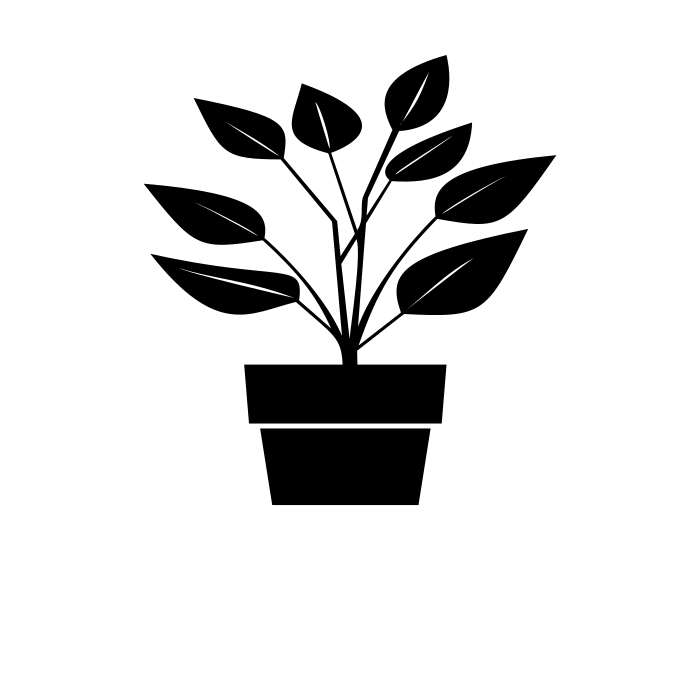
\includegraphics[width=2cm]{figures/icons-svg/noun-plant-1358991.png}
\begin{enumerate}
  \item Consider a plant you have at home (or another specific individual plant).
  \item Write a list of the factors in its environment that vary through the day.
  \item Consider the environment of roots, leaves and stems of this plant.
  \item Consider what properties of these factors are most and least important to the growth of your plant.
\end{enumerate}
\end{frame}

\section{Contents and organization of the course}

\begin{frame}{Learning objectives (in brief)}
    Are that at the end of this course:
    \begin{itemize}
    \item Learn the language of sensory and physiological ecology of plants.
    \item Learn the basic "workings" of plants and how they have adapted and how they can acclimate to environment.
    \item Learn concepts and a way of looking at plants based on the current scientific ideas.
    \item Learn how to find answers to questions about acclimation and adaptation of plants through experiments.
    \item Learn how to find, interpret and use information to solve problems and answer questions related to plant ecology.
    \item However, you will \textbf{not} have to memorize detailed information that is available in books, journals or the internet.
    \end{itemize}
\end{frame}

\begin{frame}{Contents of the course}
More details available in Moodle. All the points listed below are discussed emphasising acclimation and adaptation.
\begin{itemize}
   \item Introduction
   \item The shared environment of plants
   \item Sensory biology
   \item Adaptation and acclimation of carbon and energy metabolism
   \item Adaptation and acclimation of water uptake and loss
   \item Adaptation and acclimation to mineral nutrient supply
   \item Adaption and acclimation of morphology and anatomy
   \item Plasticity in a changing or artificial habitat
\end{itemize}
\end{frame}

%\begin{frame}{Books specially suitable for this course \Reading}
%These two easy to read books deal with subjects that I emphasise, but which have not yet made their way into traditional textbooks.
%\begin{itemize}
%    \item \citetitle{Chamovitz2013}. An excellent and accessible introduction to current understanding of the role of information in plant life \autocite{Chamovitz2013,Chamovitz2017}.
%
%    \item \citetitle{Denison2012}. An excellent and accessible discussion on the connections between evolution and agriculture, including both crop management and breeding \autocite{Denison2012}.
%\end{itemize}
%
%\end{frame}
%
%\begin{frame}{Books specially suitable for this course \Reading}
%A more advanced book emphasises subjects in this course that have not yet made their way into traditional textbooks.
%\begin{itemize}
%    \item \citetitle{Karban2015}. A thorough and balanced review of the subject. Rather advanced but still accessible \autocite{Karban2015}.
%\end{itemize}
%
%\end{frame}
%
%\begin{frame}{Books: the good ones \Reading}
%\centering
%\includegraphics[width=0.292\linewidth]{figures/Chamovitz.jpg}\hspace{0.5em}%
%\includegraphics[width=0.31\linewidth]{figures/Karban2015.jpg}\hspace{0.5em}%
%\includegraphics[width=0.31\linewidth]{figures/Denison2012.jpg}
%\end{frame}
%
%\begin{frame}{Books: the bad one \Attention}
%\centering
%Unscientific!\\ \emph{''Evidence'' given was not obtained scientifically, and results in most cases could never be independently validated.}\\ Human-like characteristics are attributed to plants.\\ \includegraphics[width=0.25\linewidth]{figures/Tompkins.jpg}
%\end{frame}
%
%\begin{frame}{Further reading in Physiological Ecology\Advanced}
%I recommend the following books for complementary reading. They are all good, but approach and focus varies significantly:
%\begin{itemize}
%  \item \citetitle{Scott2008}. Strong focus on plant-animal interactions, specially pollination \autocite{Scott2008}.
%  \item \citetitle{Lambers2008}. Book that goes in depth into physiological ecology \autocite{Lambers2008,Lambers2019}.
%  \item \citetitle{Keddy2017}. Book on plant ecology with examples from around the world \autocite{Keddy2017}.
%  \item \citetitle{Taiz2014}. Book on physiology but connections to ecology and agriculture are mentioned \autocite{Taiz2014,Taiz2018}.
%\end{itemize}
%
%\end{frame}
%
%\begin{frame}{Further reading}
%There is a book titled \citetitle{Manetas2012} \autocite{Manetas2012}, that gives a light-hearted but insightful introduction to the biology of plants. I recommend reading it to students not doing a major in plant biology.
%\end{frame}
%
%\begin{frame}{Book covers I \Advanced}
%\centering
%\includegraphics[width=0.42\linewidth]{figures/Gurevitch.jpg}\hspace{3em}%
%\includegraphics[width=0.38\linewidth]{figures/Lambers2008.jpg}
%\end{frame}
%
%\begin{frame}{Book covers II \Advanced}
%\centering
%\includegraphics[width=0.37\linewidth]{figures/Larcher.jpg}\hspace{3em}%
%\includegraphics[width=0.45\linewidth]{figures/Taiz2014.jpg}
%\end{frame}

%\section*{References}
%  \nocite{Ballare2009}
%  \begin{frame}[t,allowframebreaks]
%    \frametitle{References}
%    \printbibliography
%  \end{frame}
%
\end{document}


